\documentclass[20pt]{ctexart}
\usepackage{graphicx}
\usepackage{amsmath}
\usepackage{url}
\usepackage{subfigure}
\usepackage{float}
\usepackage{lmodern}
\usepackage{xeCJK}
\usepackage{tikz}
\usepackage{enumitem}
\usepackage{verbatimbox}
\usepackage{cite}
\usepackage{amsfonts}
\usepackage{amsthm}
\usepackage{geometry}
\usepackage{verbatimbox}
\usepackage{caption}
\usepackage{listings}
\usepackage{amssymb}
\usepackage[ruled,linesnumbered]{algorithm2e}

%设置新环境
\newtheorem{example}{例}             
\newtheorem{theorem}{定理}[section] 
\newtheorem{definition}{定义}[section]
\newtheorem{property}{性质}
\newtheorem{proposition}{命题}
\newtheorem{lemma}{引理}
\newtheorem{corollary}{推论}
\newtheorem{remark}{注}
\newtheorem{condition}{条件}
\newtheorem{conclusion}{结论}
\newtheorem{assumption}{假设}
\newenvironment{solution}{\begin{proof}[\indent\bf 解]}{\end{proof}}%设置新环境
\CTEXsetup[format={\Large\bfseries}]{section}%加入字体
\geometry{a4paper,scale=0.8}%设置文档格式
\tikzstyle{file} = [rectangle, rounded corners, minimum width = 3cm, minimum height=1.2cm ,text centered, draw = black]%设置流程图
\tikzstyle{dots} = [rectangle, rounded corners, minimum width = 1.5cm, minimum height=2cm ,text centered, draw = black,text width=3cm]%设置流程图
\tikzstyle{arrow} = [->,>=stealth]%设置流程图
\usetikzlibrary{arrows, decorations.pathmorphing, backgrounds, positioning, fit, petri, automata}%使用流程图元素
\bibliographystyle{unsrt}%设置引用格式

\title{Lab6b Report}
\author{作者:罗文杰\\专业: 计算机科学与技术\\学号: 3210102456}
\date{}

\begin{document}
\maketitle

\section{Introduction}
Write a program to execute LC-3 binary code. 
You are required to write in C or any other high level programming language.

\section{Algorithm explanation}
Basic idea: virtual machine. Language used : C.

\subsection{Program}
The flow of the procedure is as follows.
\begin{center}
        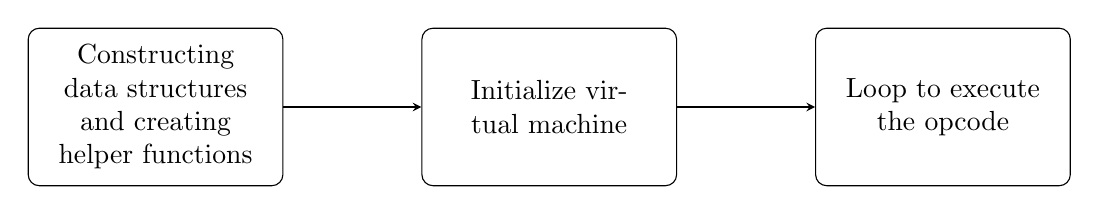
\begin{tikzpicture}[node distance = 3cm]
          \node[dots] (set1) at (-5,0) {Constructing data structures and creating helper functions};
          \node[dots] (set2) at (0,0){Initialize virtual machine};
          \node[dots] (set3) at (5,0){Loop to execute the opcode};
        
          \draw[arrow](set1) -- node[anchor=east,xshift=0.5cm,yshift=0.3cm]{}(set2);
          \draw[arrow](set2) -- node[anchor=east,xshift=0.5cm,yshift=0.3cm]{}(set3);
        \end{tikzpicture}
        \end{center}

The following is the main functions.
\begin{lstlisting}
        int main( ){
                setup(&core);
                main_loop(&core);
                return 0;
        }
        \end{lstlisting}

\subsection{Preparation}
To build a virtual machine, we first need to create a data structure, who has a uint16\_t variables to indicate Program Counter,
a two-dimensional array of length 65536 and width 16 to indicate memory locations, an array of length 8 with each cell being a unint16t variable to indicate 8 register,
and three int variables to indicate condition codes considering privilege mode and priority level are not required.
And to easierly use opcode, we create another data structure who has wwo arrays, one of size 4 and the other of size 12.
After building the data structure, construct the corresponding prototype.

In addition, we need to create the following functions before moving on to the formal program.

\begin{algorithm}[H]
	\caption{chartonum}
	\small
	\KwIn{string need to convert, number of bits to be converted}
	\KwOut{ a unsigned int }

        \While{t > 0}
        {
            temp = temp * 2 + (*str - '0');\\
            str++;\\
            t--;\\
        }
    \textbf{return} temp
\end{algorithm}

\begin{algorithm}[H]
	\caption{chartosigned}
	\small
	\KwIn{string need to convert, number of bits to be converted}
	\KwOut{ a signed int }

        temp = chartonum(str, t); \\ 
        \If{str[t]=='1'}{
                temp = chartonum(str, t); \\
        }

    \textbf{return} temp
\end{algorithm}

\begin{algorithm}[H]
	\caption{itoa}
	\small
	\KwIn{ number need to convert, conversion objectives, valuetype}
	\KwOut{ a string }
        char index[  ]="0123456789ABCDEF";\\
        \While{num > 0}
        {
                str[ i-- ]=index[ unum \% radix ];\\
                unum /= radix;\\
        }
        \For{Each character that has been constructed}
        {       
                Reverse order;\\
        }

    \textbf{return} temp
\end{algorithm}

\subsection{Initialization}
In setup, the first thing to do is to put values of all registers and memory locations to x7777.
Then, read the starting address and store it to pc. 
Finally, read each instruction in turn and place them in turn in the position after the pc.

\subsection{Loop}
In the loop, we will proceed in sequence: fetch, increment and execute.

To fetch a opcode, we need use memcpy to take the code in the address pointed by pc copy to a pointer pointering to data structure.
Then, increment the pc. And finally, execute the opcode according to bit[12:15].

The flow of each instruction is shown below.
\begin{figure}[H]
        \centering
        \includegraphics[width=0.7\textwidth]{../img/10.png}
      \end{figure}

\section{Source code}
\linespread{0.9}     
\begin{verbatim}
        \#include <stdio.h>
        \#include <stdlib.h>
        \#include <string.h>
        \#include <stdint.h>
        
        int chartonum(char* str, int t){
                ......
        }
        int chartouns(char* str, int t){
                .......
        }
        char* my_itoa(uint16_t num, char* str, int radix){
                .......
        }
        typedef struct{
            char opcode[4];
            char value[12];
        } VM_INST;
        typedef struct{
            uint16_t pc;
            int n;
            int z;
            int p;
            char rom[65536][16];
            uint16_t R[8];
        } VM_CORE;
        VM_CORE core;

        void setCondition(VM_CORE *c, uint16_t value){
            if(value == 0){
                c->n = 0;  c->p = 0;  c->z = 1;
            }else if(value & (1<<15)){
                c->n = 1;  c->p = 0;  c->z = 0;
            }else{
                c->n = 0;  c->p = 1;  c->z = 0;
            }
        }
        void do_BR(VM_CORE *c, VM_INST* inst){
            if((inst->value[0]-'0' && c->n) || 
             (inst->value[1]-'0' && c->z) || (inst->value[2]-'0' && c->p)){
                int SEXT = chartouns((char*)inst->value + 3, 9);
                c->pc += SEXT;
            }
        }
        void do_ADD(VM_CORE *c, VM_INST* inst){   
            int DR = chartonum((char*)inst->value, 3);
            int SR1 = chartonum((char*)inst->value + 3, 3);
            if(inst->value[6] == '1'){
                int SEXT = chartouns((char*)inst->value + 7, 5);
                c->R[DR] = c->R[SR1] + SEXT;
            }else{
                int SR2 = chartonum((char*)inst->value + 9, 3);
                c->R[DR] = c->R[SR1] + c->R[SR2];
            }
            setCondition(c, c->R[DR]);
        }
        void do_LD(VM_CORE *c, VM_INST* inst){
            int DR = chartonum((char*)inst->value, 3);
            int PCoffset9 = chartouns((char*)inst->value + 3, 9);
            c->R[DR] = chartonum(c->rom[c->pc + PCoffset9], 16);
            setCondition(c, c->R[DR]);
        }
        void do_ST(VM_CORE *c, VM_INST* inst){
            int SR = chartonum((char*)inst->value, 3);
            int PCoffset9 = chartouns((char*)inst->value + 3, 9);
            char * temp = malloc(sizeof(VM_INST) + 1);
            memset(temp, '0', 16);
            memcpy(c->rom[c->pc + PCoffset9], my_itoa(c->R[SR], temp, 2), 16);
            free(temp);
        }
        void do_JSR(VM_CORE *c, VM_INST* inst){
            uint16_t temp = c->pc;
            if(inst->value[0] == '1'){
                int PCoffset11 = chartouns((char*)inst->value + 1, 11);
                c->pc = c->pc + PCoffset11;
            }else{
                int BaseR = chartonum((char*)inst->value + 3, 3);
                c->pc = c->R[BaseR];
            }
            c->R[7] = temp;
        }
        void do_AND(VM_CORE *c, VM_INST* inst){
            int DR = chartonum((char*)inst->value, 3);
            int SR1 = chartonum((char*)inst->value + 3, 3);
            if(inst->value[6] == '1'){
                uint16_t SEXT = (uint16_t)chartouns((char*)inst->value + 7, 5);
                c->R[DR] = c->R[SR1] & SEXT;
            }else{
                int SR2 = chartonum((char*)inst->value + 9, 3);
                c->R[DR] = c->R[SR1] & c->R[SR2];
            }
            setCondition(c, c->R[DR]);
        }
        void do_LDR(VM_CORE *c, VM_INST* inst){
            int DR = chartonum((char*)inst->value, 3);
            int BaseR = chartonum((char*)inst->value + 3, 3);
            int offset6 = chartouns((char*)inst->value + 6, 6);
            c->R[DR] = chartonum(c->rom[c->R[BaseR] + offset6], 16);
            setCondition(c, c->R[DR]);      
        }
        void do_STR(VM_CORE *c, VM_INST* inst){
            int SR = chartonum((char*)inst->value, 3);
            int BaseR = chartonum((char*)inst->value + 3, 3);
            int offset6 = chartouns((char*)inst->value + 6, 6);
            char * temp = malloc(sizeof(VM_INST) + 1);
            memset(temp, '0', 16);
            memcpy(c->rom[c->R[BaseR] + offset6], my_itoa(c->R[SR], temp, 2), 16);
            free(temp); 
        }
        void do_NOT(VM_CORE *c, VM_INST* inst){
            int DR = chartonum((char*)inst->value, 3);
            int SR = chartonum((char*)inst->value + 3, 3);
            c->R[DR] = ~c->R[SR];
            setCondition(c, c->R[DR]);    
        }
        void do_LDI(VM_CORE *c, VM_INST* inst){
            int DR = chartonum((char*)inst->value, 3);
            int PCoffset9 = chartouns((char*)inst->value + 3, 9);
            int address = chartonum(c->rom[c->pc + PCoffset9], 16);
            c->R[DR] = chartonum(c->rom[address], 16);
            setCondition(c, c->R[DR]);    
        }
        void do_STI(VM_CORE *c, VM_INST* inst){
            int SR = chartonum((char*)inst->value, 3);
            int PCoffset9 = chartouns((char*)inst->value + 3, 9);
            char* temp = malloc(sizeof(VM_INST) + 1);
            int address = chartonum(c->rom[c->pc + PCoffset9], 16);
            memset(temp, '0', 16);
            memcpy(c->rom[address], my_itoa(c->R[SR], temp, 2), 16);
            free(temp);    
        }
        void do_JMP(VM_CORE *c, VM_INST* inst){
            int BaseR = chartonum((char*)inst->value + 3, 3);
            c->pc = c->R[BaseR];
        }
        void do_LEA(VM_CORE *c, VM_INST* inst){
            int DR = chartonum((char*)inst->value, 3);
            int PCoffset9 = chartouns((char*)inst->value + 3, 9);
            c->R[DR] = (uint16_t)(c->pc + PCoffset9);
        }
        void do_OUT(VM_CORE *c, VM_INST* inst){
            int t = 0;
            for(t = 0; t<=7 ; t++) printf("R%d = x%04hX\n", t, c->R[t]);
        }

        //loop to execute
        int main_loop(VM_CORE *c){
            VM_INST *inst = malloc(sizeof(VM_INST) + 1);
            ((char*)inst)[16] = '\0';
            while(1){

            // fetch the opcode
                memcpy(inst, c->rom[c->pc], sizeof(VM_INST));

            // increment the pc 
                c->pc += 1;

            // execute
                switch (chartonum(inst->opcode, 4)){
                    case 0:{do_BR(c, inst); break;}
                    case 1:{do_ADD(c, inst); break;}
                    case 2:{do_LD(c, inst); break;}
                    case 3:{do_ST(c, inst); break;}
                    case 4:{do_JSR(c, inst); break;}
                    case 5:{do_AND(c, inst); break;}
                    case 6:{do_LDR(c, inst); break;}
                    case 7:{do_STR(c, inst); break;}
                    case 9:{do_NOT(c, inst); break;}
                    case 10:{do_LDI(c, inst); break;}
                    case 11:{do_STI(c, inst); break;}
                    case 12:{do_JMP(c, inst); break;}
                    case 14:{do_LEA(c, inst); break;}
                    case 15:{do_OUT(c, inst); return 0;}
                    default:printf("Error!\n"); exit(-1);
                }
            }
        }

        //Initialization
        void setup(VM_CORE* core){
            int t = 0;
            char temp[17] = "0111011101110111";
            for(t=0; t<65536; t++)   memcpy(core->rom[t], temp, 16);
            core->n = 0;  core->z = 0;  core->p = 0;
            core->R[0] = 30583; core->R[1] = 30583; core->R[2] = 30583; core->R[3] = 30583; 
            core->R[4] = 30583; core->R[5] = 30583; core->R[6] = 30583; core->R[7] = 30583;
            t = 0;
            char c = '\0';
            char *address = malloc(sizeof(VM_INST) + 1);
            while (t!=16){
                c=getchar();
                address[t++] = c;
            }
            address[16] = '\0';
            core->pc = (uint16_t)chartonum(address, 16);
            free(address);
            t = 0;
            while ((c=getchar())!= EOF){
                if(c!=10)vcore->rom[core->pc][t++] = c;
            }
        }
        int main(){
            setup(&core);
            main_loop(&core);
            return 0;
        }
\end{verbatim}

\end{document}
